\subsection{Archon：形式化智能体}\label{subsec:archon}

数学证明要求完全的严谨性，然而即使是专家撰写的证明也可能包含细微的缺陷，而 LLM 产生的证明更容易出现幻觉，其可靠性要低得多。为了获得值得信赖的正确性保证，我们在流程中引入了形式化验证。如果证明通过了形式化语言编译器，那么验证正确性就归结为检查顶层陈述及其支持性定义是否忠实地捕捉了预期的数学内容。

我们采用 Lean 4 作为我们的形式化语言。其社区维护的库 Mathlib 包含由 770 多名成员贡献的超过 267,000 个定理和 127,000 个定义，提供了一个成熟的基础，使得前沿数学的形式化变得可行，因为每个依赖的定义和引理最终都必须建立在现有库的基础上。

形式化智能体 \textit{Archon} 扩展了我们之前关于陈述自动形式化的工作~\cite{gao2024herald, wang2025aria}，使其能够进行完整的证明形式化：给定一个非形式证明，它生成一个 Lean 4 项目，陈述并证明目标定理及其所有支持性定义和引理，且均基于 Mathlib。
Archon 首先通过收集依赖的参考文献来初始化项目，然后形式化关键的陈述和定义，将它们组织到特定主题的文件中。它通过迭代地填补文献中省略的空白，在遇到困难时咨询非形式智能体或外部来源，并探索替代的形式化策略，直到整个项目成功编译。

在将其部署到 Rethlas 生成的证明上之前，我们在 FirstProof~\cite{abouzaid2026first}（包含 10 个当时没有公开发布解决方案的研究级问题的集合，从而避免了数据污染）上验证了 Archon。OpenAI~\cite{openai_first_proof_2026} 和 Google~\cite{feng2026aletheia} 都在这些问题上评估了他们的系统。我们根据 Mathlib 的基础设施支持和数学意义选择了问题 4 和 6；值得注意的是，Google 的 Aletheia 在这两个问题上都失败了，而 OpenAI 成功了，但需要人工监督。Archon 为这两个问题的 OpenAI 非形式证明生成了完整的形式化：问题 6 是完全自主形式化的，而问题 4 仅在一个引理的证明倾向上需要一次自然语言提示。问题 4 的形式化大约耗时 50 小时，API 成本为 \$1,200；问题 6 耗时 30 小时，成本为 \$750。\footnote{有关更多详细信息，请参阅我们的博客文章 \url{https://frenzymath.com/blog/archon-firstproof/}}\Cref{subsubsec:workflow}回顾了工作流程和架构，而\Cref{subsubsec:enhancements}描述了自最初发布以来的增强功能。

\subsubsection{系统架构与工作流设计\label{subsubsec:workflow}}

\begin{figure}[!htbp]
    \centering
    \vspace{-0.6em}

    \begin{minipage}[t]{0.49\textwidth}
        \centering
        \vspace{0pt}
        \begin{minipage}[b][5.0cm][b]{\linewidth}
            \centering
            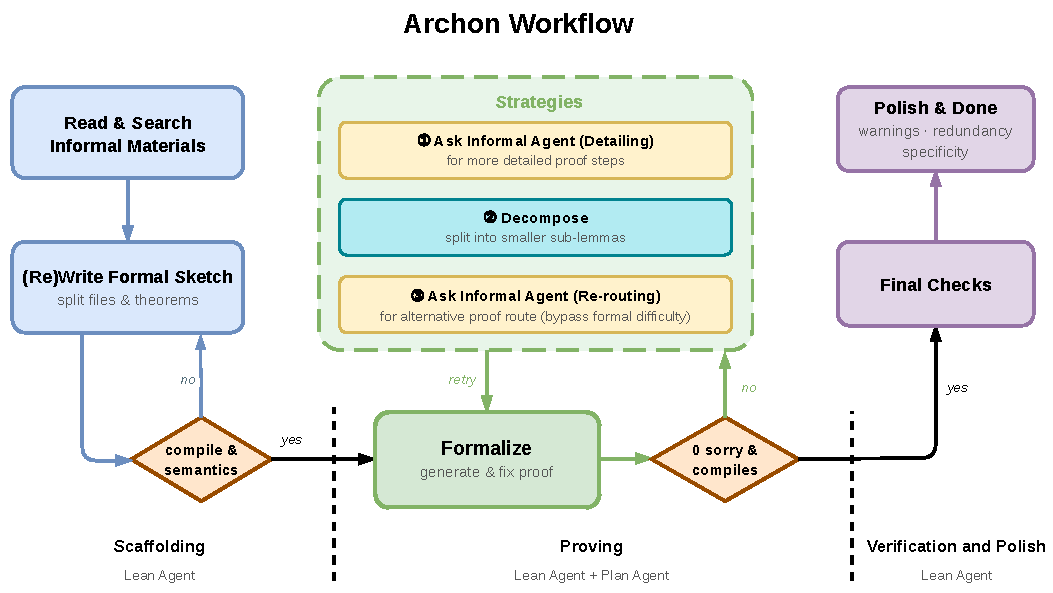
\includegraphics[
                width=\linewidth,
                height=5.0cm,
                keepaspectratio
            ]{figure/Archon_Workflow.pdf}
        \end{minipage}
        \vspace{-1.8em}
        \captionof{figure}{Archon 工作流}
        \label{fig:archon-workflow}
    \end{minipage}\hspace{0.005\textwidth}%
    \begin{minipage}[t]{0.49\textwidth}
        \centering
        \vspace{0pt}
        \begin{minipage}[b][5.0cm][b]{\linewidth}
            \centering
            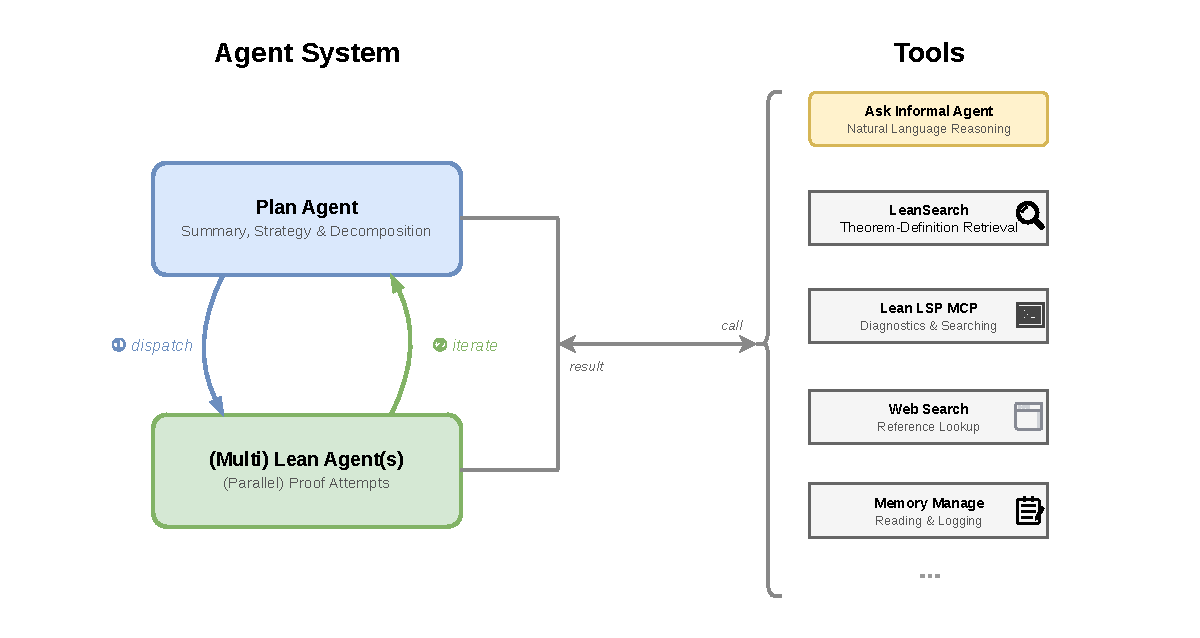
\includegraphics[
                width=\linewidth,
                height=5.0cm,
                keepaspectratio
            ]{figure/Agent_system_with_tools.pdf}
        \end{minipage}
        \vspace{-1.8em}
        \captionof{figure}{智能体系统与工具}
        \label{fig:agent-system-tools}
    \end{minipage}

    \vspace{-0.6em}
\end{figure}

我们的核心设计原则是避免硬编码的工作流，而是为智能体配备足够的技能和工具，赋予其最大的自主权。然而，我们观察到在长时间运行的会话中，特别是当智能体面临困难的引理时，累积的上下文会降低性能：智能体自身的失败尝试和悲观注释会削弱其坚持下去的意愿。为了解决这个问题，我们引入了一种双智能体架构，包括一个\textbf{规划智能体（Plan Agent）}（在一个全新的上下文中运行，用于分解任务并提供针对性的指导）和一个\textbf{Lean 智能体（Lean Agent）}（在一个受限的范围内执行形式化）。这种分离显著减轻了上下文污染和任务厌恶（例如，包含累积失败的上下文被观察到与智能体在困难义务上的坚持度降低相关）。

形式化过程分为三个阶段（\Cref{fig:archon-workflow}）：
\begin{enumerate}
    \item \textbf{搭建脚手架（Scaffolding）。} Lean 智能体分析非形式证明并构建初始文件结构：将证明拆分为模块，定义定理签名，并在每个证明义务处放置 \texttt{sorry} 占位符。这种分解不是固定的，可能会随着证明的发展而修改。
    \item \textbf{证明（Proving）。} Lean 智能体和规划智能体进入一个迭代循环。Lean 智能体尝试消除 \texttt{sorry} 占位符；当遇到困难时，它会将诊断信息返回给规划智能体，规划智能体会重新评估证明策略并分发修改后的任务。当分解产生独立的证明义务时，多个 Lean 智能体可以并行运行。
    \item \textbf{验证和打磨（Verification and Polish）。} 系统确认成功编译，并且不存在 \texttt{sorry}、\texttt{axiom} 等逃生通道，然后执行质量检查以提取可重用的引理并降低证明复杂性。
\end{enumerate}

如\Cref{fig:agent-system-tools}所示，智能体配备了一套通过终端 CLI 和模型上下文协议（MCPs）实现的工具。我们强调两个对 Archon 有效性特别重要的工具：

\textbf{咨询非形式智能体。} 当 Lean 智能体需要超出所提供的非形式证明涵盖范围的数学指导时，它会委托给非形式智能体以获取自然语言的子证明或替代策略。在大多数情况下，这是一个轻量级的 Gemini API 调用以进行快速推理。当智能体遇到更实质性的障碍时，它可能会调用 Rethlas 进行更深入、长期限的推理。

\textbf{LeanSearch。} 我们之前发布并在 Lean 社区广泛采用的检索工具，提供了对 Mathlib 定理和定义的模糊搜索。对于 Archon，我们进一步提高了它的检索准确性，并将其更新到最新的 Lean 和 Mathlib 版本。至关重要的是，LeanSearch 使智能体能够可靠地确定 Mathlib 中是否已经存在所需的结果，从而允许它在何时调用库引理和何时从头开始形式化做出充分知情的决策。这种能力对于产生充分利用现有基础设施的形式化至关重要。

其他工具包括用于编译诊断的 Lean LSP MCP、用于检索已发表参考文献的 Web 搜索，以及一个内存管理系统，该系统在上下文压缩和会话重启之间持久保存智能体的架构推理、失败的方法和学习到的技术。

仅仅提供工具是不够的；模型还需要关于何时以及如何部署它们的明确指导。这种行为指导编码在\textbf{技能（skills）}中，这些技能是建立在 Lean 4 技能框架上的结构化指令文件，它们塑造了智能体的工作模式和边界情况处理，以反映真实的形式化实践。







\subsubsection{用于猜想形式化的增强功能\label{subsubsec:enhancements}}

用于 FirstProof 问题 4 和 6 的 Archon 版本验证了双智能体架构：规划智能体在很大程度上消除了 Lean 智能体停滞或拒绝推进的情况。然而，扩展到更难的问题揭示了两个进一步的挑战。首先，随着数学难度和项目复杂性的增长，智能体偶尔会忘记先前的尝试，反复探索相同的死胡同，浪费计算资源。其次，随着项目扩大，智能体必须管理不断增加的非形式参考资料体，并且在需要时可能难以找到它们。我们引入了两个已开源的增强功能来解决这些问题。

\textbf{内存系统和复查智能体（Review Agent）。} 我们缩短了每个 Lean-Plan 迭代的持续时间，并要求每个智能体记录其会话的摘要。跨会话维护了几个全局状态文档，跟踪总体工作流阶段、每个文件的证明状态，以及局部 \texttt{sorry} 消除和重构工作的详细记录。此外，一个\textbf{复查智能体}在每个会话边界运行，以综合最近会话的趋势。这种多会话视角对于检测停滞（仅表现为连续会话的模式）至关重要。虽然复查智能体不改变形式化本身，但它使规划智能体能够在正确的时间调整策略，并为人类专家提供更清晰的进度视图。

\textbf{结构化提示和参考文献管理。} 我们将智能体的指导和参考材料重新组织成清晰的目录结构。在项目初始化期间，人类专家（在智能体的协助下）准备论文参考资料，然后智能体通过搜索添加进一步的参考资料。在面临数学困难时，智能体咨询非形式智能体，然后将候选的证明路线记录在与原始参考资料截然不同的专用位置。控制智能体工作模式和约定的技能和提示可以按项目进行自定义；在我们的实验中，当非形式参考步骤被认为是可信的时，明确指示规划智能体遵循这些步骤，显著减少了在没有前途的替代方案上花费的时间。这种设计还保持了上下文的整洁：智能体仅加载与当前任务相关的材料，避免被无关信息分心。

\medskip
\noindent 这些设计选择在\Cref{sec:archon_results}中描述的全规模形式化中起着核心作用。

\section{开放问题及 Rethlas 的解答}\label{sec:rethlas_results}

框架建立后，我们现在将注意力转移到目标数学问题上。\Cref{subsec:open_problem}介绍了背景和 Anderson 的开放问题。\Cref{subsec:nl_proof_sketch}然后给出了 Rethlas 生成的证明的概述。最后，\Cref{subsec:discovery}追溯了产生证明的逐步发现过程。

\subsection{Anderson 的开放问题}\label{subsec:open_problem}


设 \((R, \mathfrak{m})\) 为诺特局部环。回顾以下定义：
\begin{enumerate}[leftmargin=*]
    \item $R$ 被称为是 \emph{拟完备的（quasi-complete）}，如果对于 $R$ 的理想的每一个递降序列 $\{A_n\}_{n\ge 1}$ 以及每一个整数 \(k \ge 1\)，存在 \(s_k\) 使得
    \[
    A_{s_k} \subseteq \Bigl(\bigcap_{n\ge 1} A_n\Bigr) + \mathfrak{m}^k.
    \]

    \item $R$ 被称为是 \emph{弱拟完备的（weakly quasi-complete）}，如果上述条件对于满足 \(\bigcap_{n \ge 1} A_n = 0\) 的所有递降序列都成立；在这种情况下，该条件简化为
  \[
  A_{s_k} \subseteq \mathfrak{m}^k.
  \]
\end{enumerate}

这些性质自然产生于对局部环拓扑的研究。拟完备显然蕴含弱拟完备，而每一个完备局部环都是拟完备的这一推论最初是由 Chevalley 证明的 \cite[Lemma 7]{chevalley1943theory}。D. D. Anderson 提出了以下问题：

\begin{problem*}[{D. D. Anderson, \cite[Problem 8a]{cahen2014open}}]
对于诺特局部环，弱拟完备是否蕴含拟完备？
\end{problem*}

我们指派 Rethlas 去探索两种可能性：弱拟完备是否总是蕴含拟完备，或者存在一个反例。以下由 Rethlas 证明并由 Archon 在 Lean 中形式化的定理，通过构造这样一个反例提供了一个否定的回答。

\begin{theorem}\label{thm:main}
    存在一个不是拟完备的弱拟完备环。
\end{theorem}

\subsection{数学证明概述}\label{subsec:nl_proof_sketch}

%%% 并不复杂，讲述构造，定性这是一个使用了另一个领域技术性定理的证明

由 Rethlas 发现并由 Archon 形式化的反例很大程度上依赖于 Matlas 定位到的 Jensen 的一篇外部论文 \cite{jensen2006completions} 中的一个技术结果。如果没有领域专业知识，这个结果很难被发现，乍一看也并不明显相关。在这一领域已经发展了大量的研究，研究完备化和一般形式纤维（generic formal fibers）；例如，参见 \cite{heitmann1993characterization, loepp1997constructing, jensen2006completions, fleming2019completely}。然而，Rethlas 迅速识别出相关结果并成功应用了它。

有关详细的数学构造和证明，请参见附录~\ref{app:math_proof}；我们在这里仅提供一个简短的概述以澄清逻辑结构和 Jensen 结果的作用。在初步化简并应用相关文献中的几个引理之后，只需构造一个环 \(A\)，其完备化 \(T = \widehat A\) 满足以下条件：
\begin{enumerate}[leftmargin=*]
\item[A.] \(A\) 的一般形式纤维（即 \(\operatorname{Spec}\, (T \otimes_{A} \operatorname{Frac} A)\)）是平凡的。
\item[B.] 存在一个素元 \(a \in A\) 使得 \(A/aA\) 是一个不是分析不可约的（等价地，它关于极大理想的完备化不是一个整环）一维诺特局部整环。
\end{enumerate}

在这一点上，Jensen 的结果 \cite[Corollary 2.4]{jensen2006completions} 变得相关。Jensen 在温和的假设下，完全刻画了一个环 \(T\) 何时可以被实现为具有平凡一般形式纤维的局部 UFD（唯一分解整环）\(A\) 的完备化。设定
\[
T = \mathbb{C}[[x,y,z]]/(x^2 - yz)
\]
并验证 \(T\) 满足 Jensen 定理中的所有条件，从而产生所需的构造。由于 \(T\) 不是析因的，并且包含一个非主的高为一的素理想 \(Q\)，所以收缩 $q \coloneqq Q \cap A = (a)$ 产生了一个不是弱拟完备的商 \(A/aA\)。

\subsection{Rethlas 的发现过程}\label{subsec:discovery}

在本节中，我们展示 Rethlas 的发现过程，如\Cref{fig:rethlas_exploration}所示，它追溯了从\Cref{thm:main}中所述的最初问题到完整证明的旅程。

\begin{figure}[hptb]
\centering
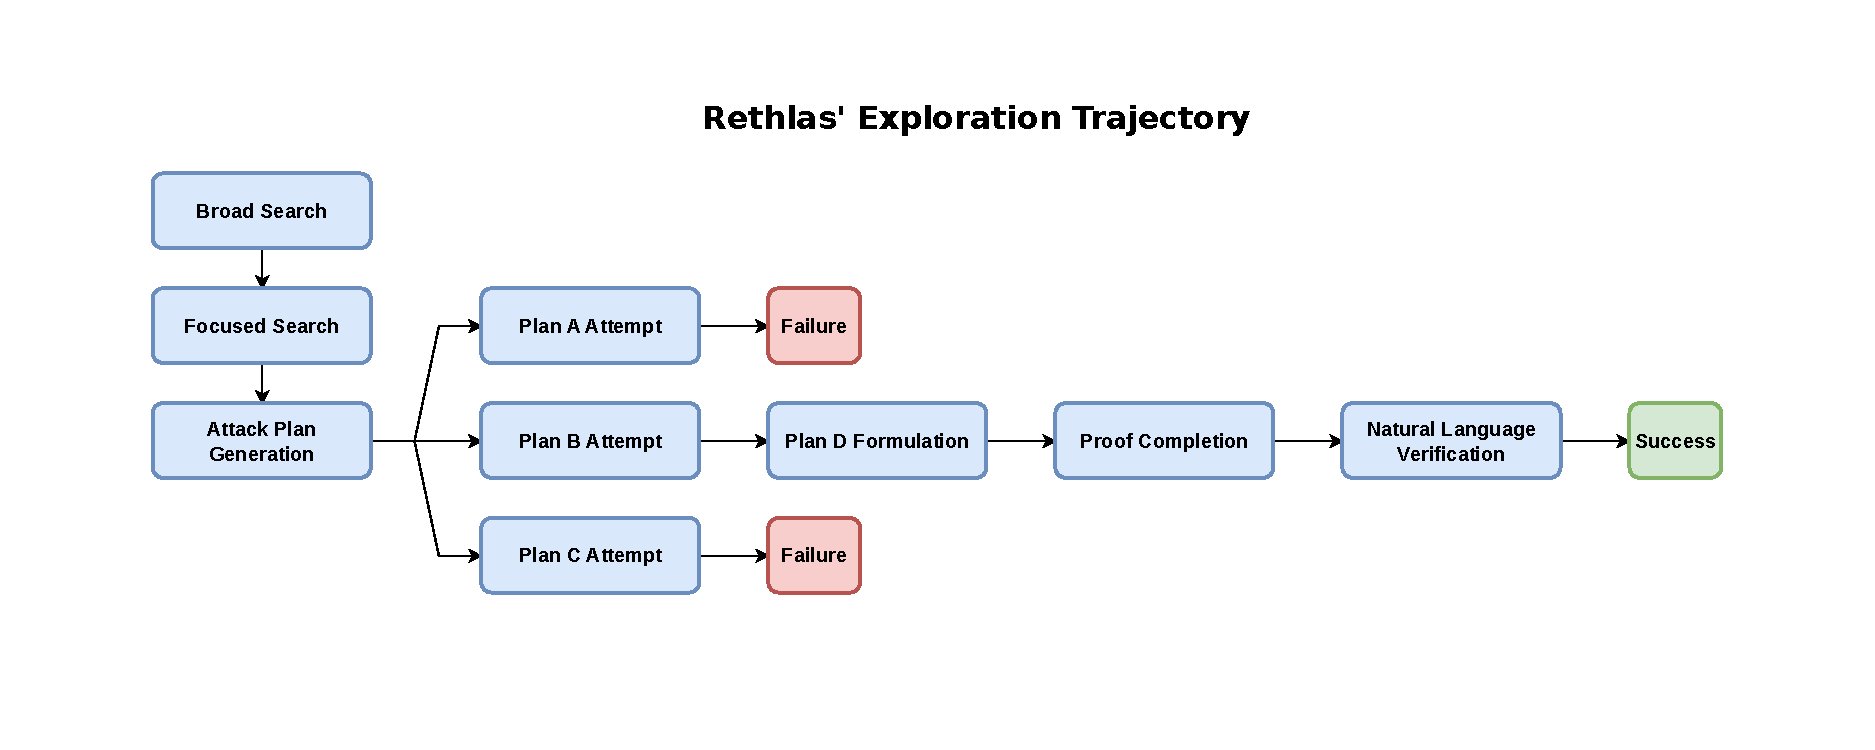
\includegraphics[width=\linewidth]{figure/rethlas_exploration_trajectory.pdf}
\caption{Rethlas 探索轨迹图示。}
\label{fig:rethlas_exploration}
\end{figure}

\begin{enumerate}[leftmargin=*]
    \item \textbf{广泛搜索。} 通过搜索最初的问题陈述及其参考文献，Rethlas 定位了将此问题记录为开放问题的文献，以及直接相关的技术资源，包括 \cite{cahen2014open, farley2016quasi}。这带来了一个更易于处理的重新表述：只需构造一个弱拟完备的环，它存在一个不是弱拟完备的同态象。
    \item \textbf{聚焦搜索。} 搜索上一步中重新表述的问题和相关结果，Rethlas 积累了进一步的技术理解。在此阶段，通过使用 Matlas 搜索查询 \verb`There exists a` \verb`weakly quasi-complete local ring with a quotient isomorphic to k[X,Y]_(X,Y).`，它发现了系统研究诺特局部环及其完备化之间关系（特别是关于一般形式纤维）的工作之一，即 \cite{fleming2019completely}。Rethlas 注意到，这一系列研究可能有助于构造所需的反例。
    \item \textbf{生成攻击计划。} 凭借从搜索结果中获得的知识，Rethlas 起草了三个分解计划来攻克这个问题。
    \begin{enumerate}[leftmargin=*]
        \item[A.] 构造一个弱拟完备环 \(R\)，它通过平方零扩张或理想化满射到一个已知的非弱拟完备局部环 \(S\)（理想情况下 \(S = k[X,Y]_{(X,Y)}\)）。
        \item[B.] 使用形式纤维控制构造一个弱拟完备局部整环 \(A\)，然后选择一个非素理想 \(I\)，使得商 \(A/I\) 的完备化表现出对弱拟完备性的明显阻碍。
        \item[C.] 从一个非弱拟完备的局部环 \(S\) 和一个具有极大理想 \(M\) 的弱拟完备扩环 \(T\) 开始。形成 \(T\) 的子环 \(R = S + M\) 或纤维积，并测试添加的 \(M\) 部分是否迫使 \(R\) 中具有零交集的每一个降链进入极大理想的幂。
    \end{enumerate}
    \item \textbf{尝试计划 A、B、C 并制定计划 D。} 计划 A 和 C 在几次尝试后失败，没有取得明显进展。在这些尝试中，继续研究将诺特局部环 \(A\) 与其完备化 \(T\) 联系起来的工作，使得 Jensen 的结果 \cite{jensen2006completions} 浮出水面。在此基础上，Rethlas 确定了一个具体的候选者 \(T = \mathbb{C}[[x,y,z]]/(x^2 - yz)\)，并提出了计划 D，它比计划 B 清晰得多。
    \begin{enumerate}[leftmargin=*]
        \item[D.] 使用 Jensen 的推论构造一个弱拟完备的局部 UFD \(A\)，其完备化 \(T\) 不是析因的，并且包含一个非主的高为一的素理想 \(Q\)；然后收缩 \(q = Q \cap A = (a)\) 产生一个不是弱拟完备的商 \(A/aA\)。
    \end{enumerate}
    \item \textbf{证明完成与验证。} Rethlas 算出了剩余的证明细节，并生成了一个 Markdown 文件，该文件清楚地陈述了所有引用的定理和论证的逻辑步骤。自然语言验证器接受了该证明，产生了最终输出。一些人类数学家认为可以忽略但形式化验证要求的一些次要细节并未完全填补；参见附录~\ref{subsubsec:gap-filling}。
\end{enumerate}

\section{形式化与验证}\label{sec:archon_results}

有了非形式证明在手，我们现在转向它在 Lean 4 中的形式化和验证。由 Archon 执行的形式化\footnote{完整的形式化代码开源在 \url{https://github.com/frenzymath/Anderson-Conjecture}。}，将 Anderson 猜想的完整证明翻译成了基于 Mathlib 的 Lean 4 项目，涵盖了主定理、所有支持性引理以及从六篇外部论文中提取的关键结果。这项任务绝非易事：除了常规的翻译之外，形式化还需要填补非形式论证中留下的隐含空白，以完整的细节实现未充分指定的构造（如超限递归），并调整证明策略以适应可用的库基础设施。根据对 Mathlib 贡献者的采访，我们估计一位经验丰富的形式化专家每天大约能产生 150-250 行 Lean 代码；因此，Archon 产生的 19,000 行代码库代表了相当于专家几个月工作量的工作负荷，在大约 80 小时的运行时间内自主完成。

我们首先对形式化输出及其关键的定量和定性特征进行概述（\Cref{subsec:overview-result}），然后讨论在此过程中吸取的经验教训和观察到的局限性（\Cref{subsec:lessons}）。

